   Para melhor visualização dos fenômenos previamente expostos, foram elaboradas simulações pertinentes para análise de sistemas de mecânica celeste \cite{sashalag, sashaeng} -- utilizando a linguagem C++. Trata-se de um sistema fictício de duas partículas de massas $M_1 = 10^{12}$ e $M_2 = 10^{10}$ unidades de massa e distância inicial da ordem $10^6$ unidades de distância. Uma terceira partícula de massa $10^2$ unidades de massa é então inserida em cada um dos pontos de Lagrange por vez, com o intuito de verificar a evolução temporal do sistema. A simulação é iniciada com $M_1$ e $M_2$ no eixo horizontal com respectivas velocidades $(0,0)$ e $(0, 10^6)$. A velocidade inicial da terceira partícula foi apropriadamente escolhida para um melhor acoplamento orbital em cada ponto de Lagrange, a saber: $(0,1,083942 \cdot 10^6)$ para L1, $(0,9,329572 \cdot 10^5)$ para L2, $(0,-9,978991 \cdot 10^5)$ para L3, $(-8,68161\cdot 10^5, 5,01233 10^5)$ para L4 e $(8,68161\cdot 10^5, 5,01233 \cdot 10^5)$ para L5. Os resultados, dispostos nas imagens a seguir, variam de acordo com os pontos analisados em cada uma das simulações apresentadas nas respectivas imagens, as partículas de massa $10^2$ são grafadas por $P_{N}$ com seus respectivos pontos de Lagrange $L_{N}$, com $N = 1,..., 5$. 
   
\begin{figure}[h]
\centering
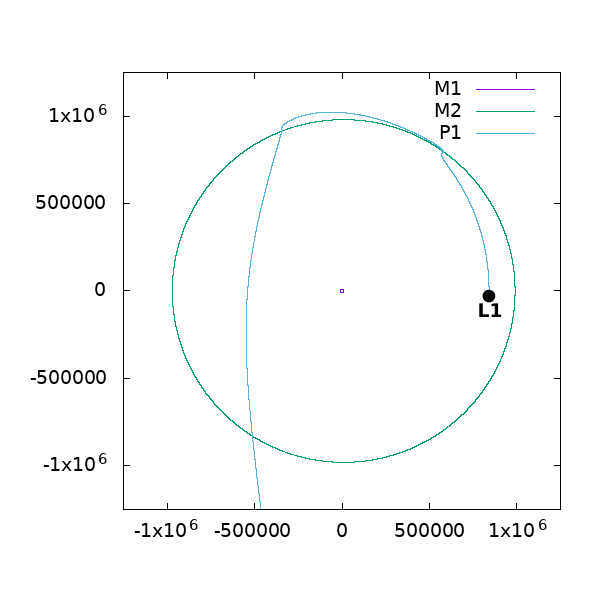
\includegraphics[width = 3 in]{./sim/L1-final.png}
\caption{O ponto grafado como L1 é a posição do ponto de Lagrange 1 no instante inicial. Trata-se de um ponto instável.}
\end{figure}

\begin{figure}[h]
\centering
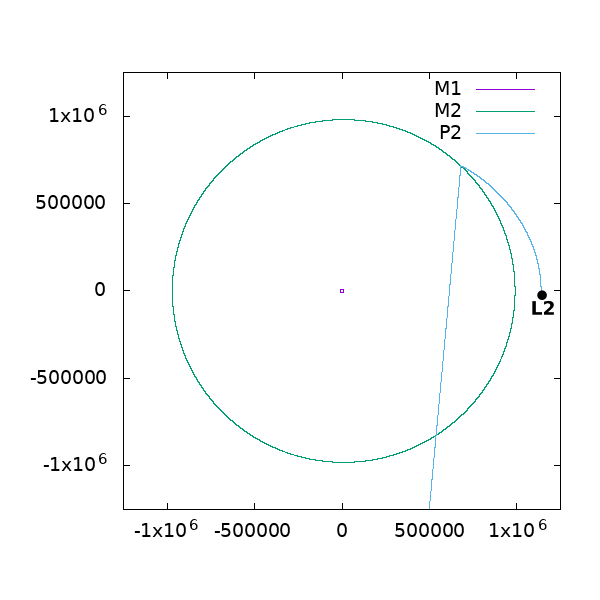
\includegraphics[width = 3 in]{./sim/L2-final.png}
\caption{O ponto grafado como L2 é a posição do ponto de Lagrange 2 no instante inicial. Trata-se de um ponto instável.}
\end{figure}

\begin{figure}[H]
\centering
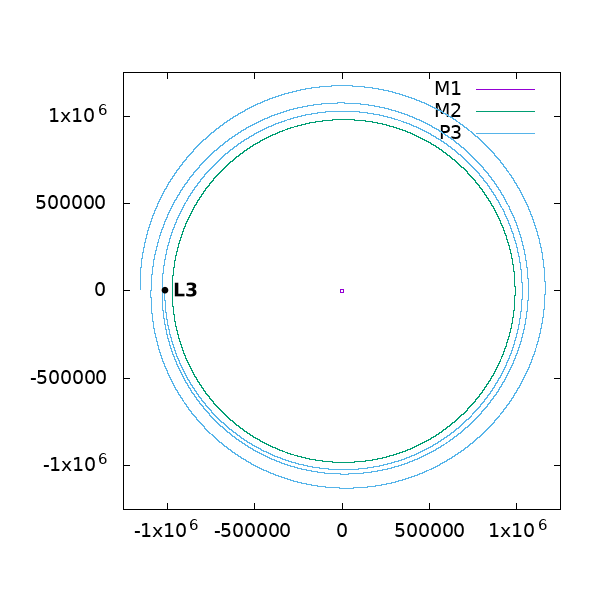
\includegraphics[width = 3 in]{./sim/L3-final.png}
\caption{O ponto grafado como L3 é a posição do ponto de Lagrange 3 no instante inicial. Trata-se de um ponto instável.}
\end{figure}

\begin{figure}[H]
\centering
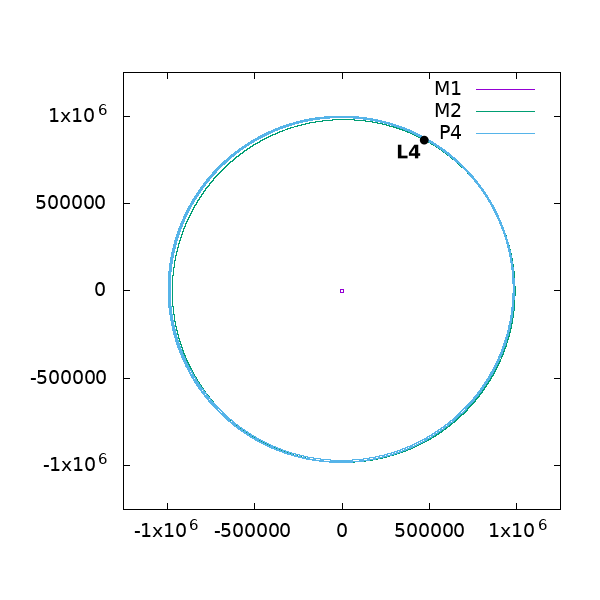
\includegraphics[width = 3 in]{./sim/L4-final.png}
\caption{O ponto grafado como L4 é a posição do ponto de Lagrange 4 no instante inicial. Trata-se, nesse caso, de um ponto estável.}
\end{figure}

\begin{figure}[H]
\centering
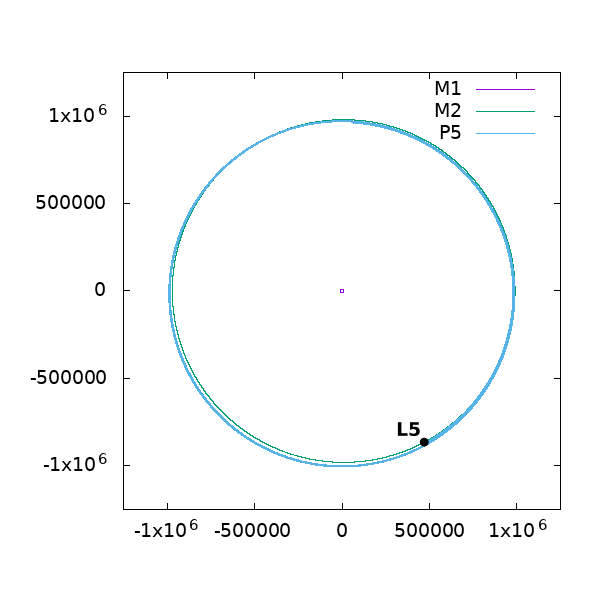
\includegraphics[width = 3 in]{./sim/L5-final.png}
\caption{O ponto grafado como L5 é a posição do ponto de Lagrange 5 no instante inicial. Analogamente a L4, temos para esse caso um ponto estável.}
\end{figure}

   A instabilidade de L1, L2 e L3 é evidenciada pela trajetória descrita pelo terceiro corpo. Ao ser acelerado pelo efeito estilingue, ele se desvia de sua órbita. Interessante notar que a órbita de P3 é consideravelmente mais estável do que as de P1 e P2, comportamento esperado pelo autovalor descrito no capítulo 2. Por outro lado, em L4 e L5, podemos observar órbitas bem comportadas, o que configura a estabilidade dos pontos.
